\chapter{Sprzęt wykorzystany w projekcie}
\label{cha:Zybo_PCAM_dron}


\section{Platforma obliczeniowa}
\label{sec:platforma_obliczeniowa}
%TODO2 W sumie zdjęcie ZYBO nie zaszkodzi, ale takie nie na pół storny, tylko skromniejsze

W~pracy wykorzystano platformę Digilent~Zybo~Z7-20 z~układem Zynq SoC (ang. \textit{System on Chip}) XC7Z020-1CLG400C. 
Układ dostępny na karcie określa się jako heterogeniczny tj. stanowi połączenie części rekonfigurowalnej (PL -- ang. \textit{programmable logic}) oraz systemu procesorowego z~dwurdzeniowym procesorem ARM Cortex-A9 taktowanym z~częstotliwością 667~MHz (PS -- ang. \textit{processing system}).

Na rysunku \ref{fig:zynq} przedstawiono architekturę układu Zynq SoC. 
System procesorowy zaznaczony został na~zielono, natomiast część rekonfigurowalna na~żółto. 
Część PS, oprócz dwurdzeniowego procesora ARM, zawiera wiele komponentów, między innymi:
\begin{itemize}
	\item wydajne kontrolery 1Gb Ethernet, USB 2.0, SDIO (ang. \textit{Secure Digital Input Output}),
	\item kontrolery SPI, UART, CAN, I2C,
	\item kontroler pamięci DDR3,
	\item infrastrukturę magistrali \textit{Advanced Microcontroller Bus Architecture Interconnect} (AMBA),
	\item inne kontrolery peryferiów z~wejściami/wyjściami multipleksowanymi do~54~dedykowanych pinów MIO (ang. Multiplexed Input Output),
	\item piny EMIO (ang. Extended MIO) pozwalające na podłączenie komponentów poprzez część PL.
\end{itemize}
<<<<<<< HEAD

Kontrolery peryferiów są podłączone do~części PS poprzez magistralę AMBA w~trybie \textit{slave}. 
W~ten sposób uzyskują dostęp do~rejestów odczytu/zapisu, adresowalnych w~pamięci procesora. 
Również część rekonfigurowalna jest połączona z~magistralą AMBA poprzez porty AXI jako \textit{slave}. 
Daje to~możliwość szybkiej komunikacji między układem FPGA, a~procesorem. 
Ponadto, moduły zaimplementowane w~części PL mogą wywoływać przerwania w~procesorze i~otrzymywać dostęp DMA (ang. \textit{Direct Memory Access}) do~pamięci DDR3.
%TODO2 proszę doczytać, bo slave to są te General Purpose, a pozostałe są master. Tzn. nie musi Pan tego rozkmniać, ale trzeba dopisać, że master też.

=======
\begin{figure}[h]
	\centering
	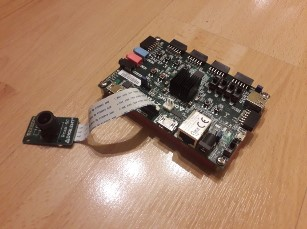
\includegraphics[width=0.5\textwidth]{plytka_kamera.jpg}
	\caption{Układ ZYBO~Z7-20 wraz z~kamerą PCAM~5C.}
	\label{fig:plytka_kamera}
\end{figure}
Kontrolery peryferiów są podłączone do~części PS poprzez magistralę AMBA w~trybie \textit{slave}. W~ten sposób uzyskują dostęp do~rejestów odczytu/zapisu, adresowalnych w~pamięci procesora. Również część rekonfigurowalna jest połączona z~magistralą AMBA poprzez porty AXI jako \textit{slave}. Daje to~możliwość szybkiej komunikacji między układem FPGA, a~procesorem. Ponadto, moduły zaimplementowane w~części PL mogą wywoływać przerwania w~procesorze i~otrzymywać dostęp DMA (ang. \textit{Direct Memory Access}) do~pamięci DDR3.\par
%TODO potem to zdanie, nieco przeredagowane.
>>>>>>> 65f53b1db22d3a9ab1904ccaf9af33bb2165b4c7
%Do dyspozycji projektanta pozostawało 53 200 tablic LUT (ang. \textit{Look-up Table}), 106 400 przerzutników \textit{flip-flop} oraz 630 KB pamięci blokowej RAM.
Poniżej przedstawiono komponenty części rekonfigurowalnej:
\begin{itemize}
	\item 53 200 tablic LUT (ang. \textit{Look-up Table}),
	\item 106 400 przerzutników \textit{flip-flop},
	\item 630 KB pamięci blokowej RAM,
	\item 6 obszarów zarządzania zegarami CMT (ang. \textit{Clock Management Tiles}),
	\item konwerter analogowo-cyfrowy.
\end{itemize}
Do pozostałych części układu ZYBO Z7-20 należą między innymi:
\begin{itemize}
	\item łącznik kamery PCAM ze wsparciem MIPI CSI-2,
	\item wejściowy oraz wyjściowy port HDMI,
	\item slot na kartę SD,
	\item 6 portów PMOD,
	\item 4 przełączniki,
	\item 5 diod LED.
\end{itemize}

%TODO2 Rysunek nieco mniejszy i może jakoś wcześniej (bliżej opisu)
\begin{figure}[h]
	\centering
	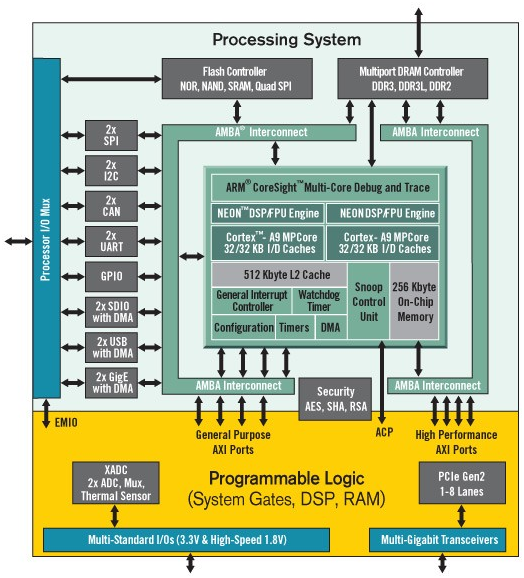
\includegraphics[width=\textwidth]{zynq.png}
	\caption{Architektura układu Zynq SoC \cite{zynq}.}
	\label{fig:zynq}
\end{figure}


\section{Moduł rejestrujący obraz}
\label{sec:pcam}
<<<<<<< HEAD

W~projekcie wykorzystano kolorową kamerę Digilent~PCAM~5C. 
Jest to~moduł przeznaczony do~użycia z~dedykowanymi płytkami rozwojowymi firmy Digilent. 
Jednym z~kompatybilnych układów jest ZYBO Z7-20. 
Podstawowe parametry modułu przedstawiono poniżej:
=======
W~projekcie wykorzystano kolorową kamerę Digilent~PCAM~5C. Jest to~moduł przeznaczony do~użycia z~dedykowanymi płytkami rozwojowymi. Jednym z~kompatybilnych układów jest ZYBO Z7-20. Na~Rys.~\ref{fig:plytka_kamera} przedstawiono kamerę podłączoną do~układu. Właściwości modułu przedstawiono poniżej:
>>>>>>> 65f53b1db22d3a9ab1904ccaf9af33bb2165b4c7
\begin{itemize}
	\item Rozdzielczość: 5 megapikseli,
	\item Matryca: OV5640,
	\item Interfejs danych: MIPI CSI-2,
	\item Złącze: 15-pinowe FFC.
\end{itemize}

%TODO2 Zdjęcie ? Ilustracja ? Może ew. obok tego Zybo, bo powinno się ładnie zmieścić.

Sposób podłączenia kamery i~układu ZYBO Z7-20 przedstawione zostały w~podrozdziale \ref{sec:integracja_uklad_kamera}.

\section{Platforma statku powietrznego}
\label{sec:platforma_statku_powietrznego}

W~projekcie wykorzystano dron sześciowirnikowy, znajdujący się na~wyposażeniu Studenckiego Koła Naukowego AVADER. 
Jego budowa była częścią innego projektu \cite{mgr}. 
Komponenty używanego bezzałogowago statku powietrznego to:
\begin{itemize}
	\item rama DJI F550,
	\item śmigła o średnicy równej 22,86~cm oraz skoku 12,7~cm,
	\item silniki DJI 2312/960KV z kontrolerami 420 LITE,
	\item czterokomorowa bateria LiPo o nominalnym napięciu 14,8~V i~pojemności 6450mAh, 
	\item nadajnik radiowy FrSky Taranis X9D Plus, odbiornik FrSky X8D,
	\item sterownik 3DR Pixhawk.
\end{itemize}

\section{Sterownik drona}
%TODO2 Fotos ?
\label{sec:autopilot}
Urządzeniem bezpośrednio komunikującym się z~kontrolerami silników jest sterownik. 
W~pracy wykorzystano urządzenie Pixhawk -- popularny kontroler lotu ogólnego przeznaczenia, który jest dostępny na~otwartej licencji. %TODO2 a nie raczej jego obprogramowanie
Jego główne parametry~to:
\begin{itemize}
	\item procesor Cortex-M4F z zegarem 168 MHz,
	\item czujniki: akcelerometr, żyroskop, kompas magnetyczny, barometr i~zewnętrzny moduł GPS,
	\item interfejsy: UART, CAN, I2C, SPI,
	\item wejście karty SD,
	\item zewnętrzny przełącznik bezpieczeństwa uzbrajania,
	\item wielokolorowa dioda pokazująca stan pracy.
\end{itemize}
Konfiguracja sterownika jest możliwa przy użyciu programu \textit{Mission Planner}. 
Jest to~aplikacja przeznaczona dla~stacji naziemnej umożliwiająca:
\begin{itemize}
	\item strojenie czujników autopilota,
	\item monitorowanie stanu sterownika (uzbrojenie silników, orientacja statku powietrznego),
	\item planowanie, zapisywanie i~wgrywanie planów autonomicznych misji statku powietrznego,
	\item pobieranie i~analizowanie dzienników misji.
\end{itemize} 

Po~instalacji oprogramowania ArduPilot sterownik umożliwia pracę w~różnych trybach. 
Dostępne są~23 tryby wbudowane, z~czego 5 jest rekomendowanych \cite{pixhawk_modes}. 
Istnieją tryby wspierające różne poziomy i~typy stabilizacji, a~zadania wykonywane przez autopilota w~każdym z~nich nieco się różnią. 
Poniżej przedstawiono podsumowanie najważniejszych cech rekomendowanych trybów:
\begin{itemize}
	\item \textit{Stablize} -- pozwala operatorowi na~manualne sterowanie dronem, stabilizując jego pochylenie i~przechylenie,
	\item \textit{Alt Hold} -- kontroluje ustawienie mocy silników w~celu utrzymania wysokości,
	\item \textit{Loiter} --  utrzymuje aktualną pozycję drona, jeśli operator nie wydaje żadnych poleceń,
	\item \textit{Return-To-Launch} --  dron unosi się na~domyślną wysokość 15~metrów, a~następnie powraca do~miejsca, w~którym został uzbrojony. Tryb ten wymaga sygnału GPS,
	\item \textit{Auto} --  dron realizuje zaprogramowaną wcześniej misję, poruszając się po~zdefiniowanych punktach. Wymagany jest sygnał GPS.
\end{itemize}

Z~punktu widzenia autonomicznego lądowania, odpowiednim trybem do~sterowania dronem jest tryb \textit{Guided}.
Umożliwia on~bowiem wysyłanie dronowi komend dotyczących zmiany szybkości i~lotu w~określonym kierunku. %TODO2 nieco niejasna konstrukcja może szybkości i kierunku lotu ?
Zazwyczaj wykorzystywana jest komunikacja ze~stacją naziemną drogą radiową (przy użyciu programu Mission Planner), lecz wysyłanie komend przez urządzenie umieszczone na~platformie drona również jest możliwe.
Komunikacja taka przebiega z~wykorzystaniem protokołu MAVLink (ang. \textit{Micro Air Vehicle Link}).
Umożliwia on~przesyłanie danych i~komend z~wykorzystaniem prawie każdego rodzaju transmisji szeregowej \cite{mavlink_basics}. 
W~tabeli \ref{tab:frame} przedstawiono opis ramki protokołu.
\begin{table}[]
	\caption{Opis ramki protokołu MAVLink}
	\label{tab:frame}
	\begin{tabular}{|l|l|l|l|}
		\hline
		Indeks bajtu & Zawartość                                                                         & Wartość        & Uwagi                                                                                                                            \\ \hline
		0            & Znak początku pakietu                                                             & 0xFE           & Wskazuje na początek nowego pakietu.                                                                                             \\ \hline
		1            & Długość danych                                                                    & n (0-255)      & Informuje o liczbie przesyłanych danych.                                                                                          \\ \hline
		2            & Sekwencja pakietu                                                                 & 0-255          & \begin{tabular}[c]{@{}l@{}}Wartość zwiększana przy każdej transmisji.\\ Umożliwia detekcję utraty pakietów.\end{tabular}         \\ \hline
		3            & ID systemu                                                                        & 1-255          & \begin{tabular}[c]{@{}l@{}}ID systemu wysyłającego. Umożliwia odróżnienie\\ różnych sieci.\end{tabular}                          \\ \hline
		4            & ID komponentu                                                                     & 0-255          & \begin{tabular}[c]{@{}l@{}}ID komponentu wysyłającego. Umożliwia \\ odróżnienie różnych komponentów w jednej sieci.\end{tabular} \\ \hline
		5            & ID wiadomości                                                                     & 0-255          & \begin{tabular}[c]{@{}l@{}}Oznacza typ wiadomości i umożliwia jej\\ zdekodowanie.\end{tabular}                                   \\ \hline
		6--n+6      & Dane                                                                              & (0-255) bajtów & Zawartość wiadomości. Zależy od jej ID.                                                                                          \\ \hline
		n+7--n+8    & \begin{tabular}[c]{@{}l@{}}Suma kontrolna\\ (młodszy i starszy bajt)\end{tabular} & \multicolumn{2}{l|}{Umożliwia wykrycie błędów transmisji}                                                                                         \\ \hline
	\end{tabular}
\end{table}
<<<<<<< HEAD

Kwestię połączenia autopilota i układu ZYBO~Z7-20 opisano w~podrozdziale \ref{sec:integracja_plytka_autopilot}.

=======
\\Kwestię połączenia autopilota i układu ZYBO~Z7-20 opisano w sekcji \ref{sec:integracja_plytka_autopilot}.
\begin{figure}[h]
	\centering
	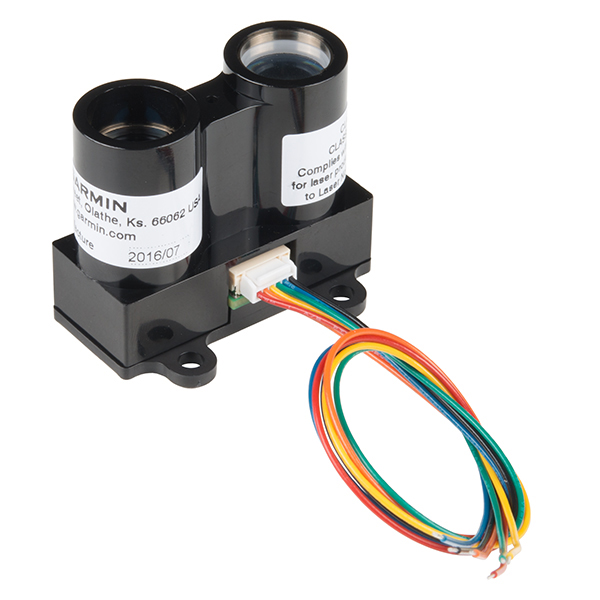
\includegraphics[width=0.4\textwidth]{lidar.jpg}
	\caption{Laserowy czujnik odległości Garmin Lidar Lite v3 \cite{lidar}}
	\label{fig:lidar}
\end{figure}
>>>>>>> 65f53b1db22d3a9ab1904ccaf9af33bb2165b4c7
\section{Laserowy czujnik wysokości}
\label{sec:laser}
W~projekcie do~pomiaru wysokości wykorzystano urządzenie Garmin Lidar Lite v3. 
Jego główne parametry~to:
\begin{itemize}
	\item Napięcie zasilania -- 5 V,
	\item Zasięg pomiaru -- 40 m,
	\item Dokładność -- 2,5 cm (pomiar do 5 m), 
	\item Wykorzystywana długość fali -- 905 nm,
	\item Interfejsy -- I2C, PWM z~zewnętrznym wyzwalaniem pomiaru.
\end{itemize}
<<<<<<< HEAD

%TODO2 Zdjęcie.

%TODO2 Proszę jeszcze opisać to radio (i zdjęcie) - nie zaszkodzi, że tam będzie. Nawet jeśli nie działa.
=======
Na~Rys.~\ref{fig:lidar} przedstawiono moduł wraz z~dołączonymi przewodami.
>>>>>>> 65f53b1db22d3a9ab1904ccaf9af33bb2165b4c7
